\documentclass[11pt]{article}
\usepackage{amsmath,amssymb,amsthm}
\usepackage{fancyhdr}
\usepackage{tikz-qtree}
\usepackage{enumerate}
\usepackage{graphicx}

% margins
\usepackage[vmargin=1in,hmargin=1.5in]{geometry}

% Config
%%%%%%%%%%%%%%%%%%%%%%%%%%%%%%%%%%%
\newcommand{\ass}{2}
\newcommand{\name}{Connor Taffe}
\newcommand{\tno}{3742} % last 4 digits of T number.
%%%%%%%%%%%%%%%%%%%%%%%%%%%%%%%%%%%

\title{
	$A_{\ass}$ \\
	{\large Assignment \ass\\
	CS 3482; Professor Tang}
}
\author{
	\name. T no. \tno
}

\pagestyle{fancy}
\rhead{Homework \ass}
\lhead{{\name}. T no. \tno}

\begin{document}
\maketitle

{\bf Notice}: I have used a format for binary number addition where extraneous places are shown when they would illustrate the generation of a $C_{\text{in}}$ bit. For example, a one bit adder might be accompanied by an example expression such as the following:

	\[
		1.1_2 + 0.1_2 = 10_2
	\]

	The topmost bit of the rightmost number in the expression is the $C_{\text{out}}$ value, and the lowest bit is the $S$ (sum) for the current bit addition. The lower bit in the operands is only shown to illustrate that a carry ($C_{\text{in}}$) bit was generated on some previous addition.

\section{Single-bit full adder}

\begin{enumerate}[(a)]
	\item{
	Show the truth table of $C$ (carry) and S(sum) of single-bit adder with input $X$, $Y$ and $C_{\text{in}}$ (carry-in) simulating the single-bit binary arithmetic addition.

		The truth table of $C$ (carry) is as follows in figure \ref{fig:1a}. C is the carry bit, so it is true if $XY$ is true ($1_2+1_2=10_2$) or if $(X \oplus Y)C_{\text{in}}$ is true ($1.1_2+0.1_2=10_2$).

		The truth table of $S$ (sum) is illustrated in the same figure. It can be seen that the sum bit is only on if $CXYC_{\text{in}} + C'(X+Y+C_{\text{in}})$ is true. This last statment is purely observational. This is because a two bits ($1_2+1_2=10_2$) rolls over to the next place (generates carry without sum bit), but three bits ($1.1_2+1.1_2=11_2$) rolls over and leaves one behind (generates carry with sum bit), and one ($0_2+1_2=1_2$) does not roll over (generates no carry, but sum bit).

		\begin{table}[h]
		\centering
		\begin{tabular}{lllll}
			$X$ & $Y$ & $C_{\text{in}}$ & $C$ & $S$ \\ \hline
			0 & 0 & 0 & 0 & 0 \\
			0 & 0 & 1 & 0 & 1 \\
			0 & 1 & 0 & 0 & 1 \\
			0 & 1 & 1 & 1 & 0 \\
			1 & 0 & 0 & 0 & 1 \\
			1 & 0 & 1 & 1 & 0 \\
			1 & 1 & 0 & 1 & 0 \\
			1 & 1 & 1 & 1 & 1 \\
		\end{tabular}
		\caption{\label{fig:1a} Truth table for $C$ and $S$ in single-bit full adder.}
		\end{table}
	}
	\item{
		Show the sum of min-term expression of $C$ and $S$.

		The minterms of $C$ are as follows:
		\[
			C_{\sum_{\text{minterm}}} = X'YC_{\text{in}} + XY'C_{\text{in}} + XYC_{\text{in}}' + XYC_\text{in}
		\]
		As we can see more clearly, two bits must be set (first three min-terms) to rollover, or all three bits (last min-term) to generate a carry and a sum.

		The minterms of $S$ are as follows:
		\[
			S_{\sum_{\text{minterm}}} = X'Y'C_{\text{in}} + X'YC_{\text{in}}' + XY'C_{\text{in}}' + XYC_\text{in}
		\]
		As we can see more clearly, only one bit can be set (first three min-terms), or three bits can be set (last min-term) for a sum bit to be on.
	}
	\item{
		Implement the single-bit full adder on LogicWorks using the following Boolean expressions:
		\[
			C = XY + XC_{\text{in}} + YC_{\text{in}}
		\]
		\[
			S = X \oplus Y \oplus C_{\text{in}}
		\]

		For illustrative purposes, here follows the parse trees of the above boolean expressions (figures \ref{fig:1c}, \ref{fig:1c2}). They can be used to show the structure of the resulting logic circuit.
		\begin{figure}[h]
			\centering
			\Tree [.$+$ [.$*$ $X$ $Y$ ] [.$*$ $X$ $C_{\text{in}}$ ] [.$*$ $Y$ $C_\text{in}$ ] ]
		\caption{\label{fig:1c} Parse tree of boolean expression for $C$.}
		\end{figure}

		\begin{figure}[h]
			\centering
			\Tree [.$\oplus$ $X$ $Y$ $C_{\text{in}}$ ]
		\caption{\label{fig:1c2} Parse tree of boolean expression for $S$.}
		\end{figure}

		Figure \ref{fig:1cc} shows the LogicWorks circuit implementation and figure \ref{fig:1ct} shows the testing of the circuit. The testing shows that the circuit is properly functioning for each of 8 inputs. It correlates to the truth table in figure \ref{fig:1a}. In the first column, $X=0,Y=0,C_{\text{in}}=0$, and $S=0,C=0$ which correlates with the truth table. The second column shows $X=0,Y=1,C_{\text{in}}=0$, and $S=1,C=0$, which correlates with the truth table. The remaining columns also correlate with the truth table, as $S$ is true only if one or three of the inputs are true, and $C$ is true only if two or three of the inputs are true, which is the same as was discussed above.

		\begin{figure}[h]
			\centering
			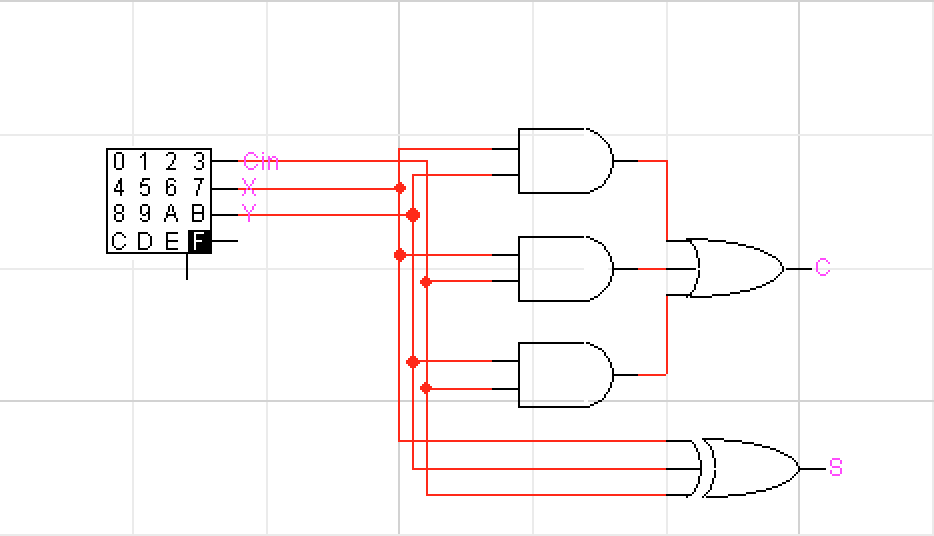
\includegraphics[width=300pt]{1c}
			\caption{\label{fig:1cc} LogicWorks circuit implementation.}
		\end{figure}

		\begin{figure}[h]
			\centering
			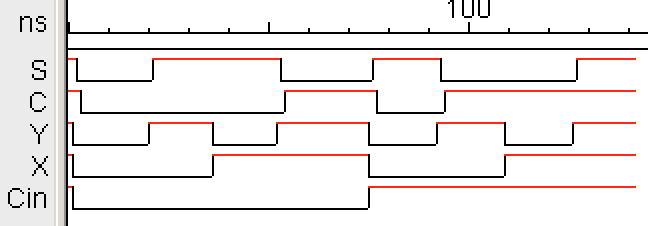
\includegraphics[width=200pt]{1t}
			\caption{\label{fig:1ct} Testing of circuit.}
		\end{figure}
	}
	\item{
	Pack your single-bit full adder and name it as {\tt fa-1}. Show the testing of your packaged single-bit full adder.

	The LogicWorks circuit is shown in figure \ref{fig:1dc}, while the testing is shown in figure \ref{fig:1dt}. The $C_{\text{in}}$, $X$, and $Y$ inputs are tested in the same order as the previous test, and we can see that it has the exact same output for $S$ and $C$. Since we have established that the output for the previous testing was correct, this packaged circuit must also be correct.

		\begin{figure}[h]
			\centering
			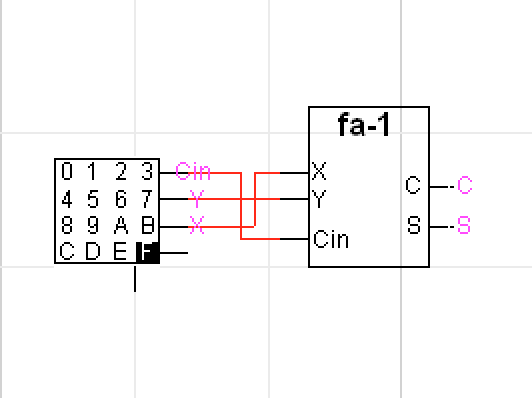
\includegraphics[width=200pt]{1pc}
			\caption{\label{fig:1dc} LogicWorks circuit implementation.}
		\end{figure}

		\begin{figure}[h]
			\centering
			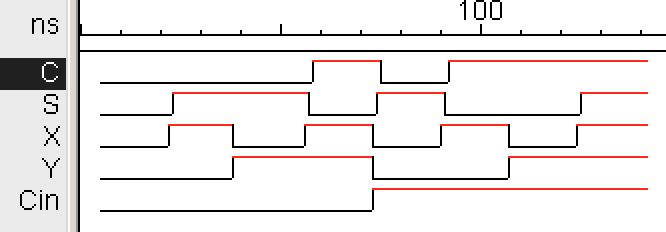
\includegraphics[width=200pt]{1pt}
			\caption{\label{fig:1dt} Testing of circuit.}
		\end{figure}
	}
\end{enumerate}

\section{Ripple carry binary adder}

\begin{enumerate}[(a)]
	\item{
		Implement a 4-bit ripple carry binary adder with inputs $A_{3\text{-}0}$, $B_{3\text{-}0}$ and $C_{\text{in}}$ and outputs $S_{3\text{-}0}$ and $C_{\text{out}}$, using the singe-bit full adder you built in the previous question. Show three test cases to demonstrate that your adder works correctly (You need to do binary add yourself and then show that your adder delivers the correct result, for each of the three input cases).

		The three cases for testing are as follows:
		\begin{enumerate}[1.]
			\item{
				\[
					1010.1_2 + 1100.1_2 = 10111_2
				\]
				\[
					C_{\text{in}} = 1,
					A_0 = 0, A_1 = 1, A_2 = 0, A_3 = 1,
					B_0 = 0, B_1 = 0, B_2 = 1, B_3 = 1,
				\]
				\[
					S_0 = 1, S_1 = 1, S_2 = 1, S_3 = 0, C_{\text{out}} = 1
				\]

				Testing shown in figure \ref{fig:2atc}.

				\begin{figure}[h]
					\centering
					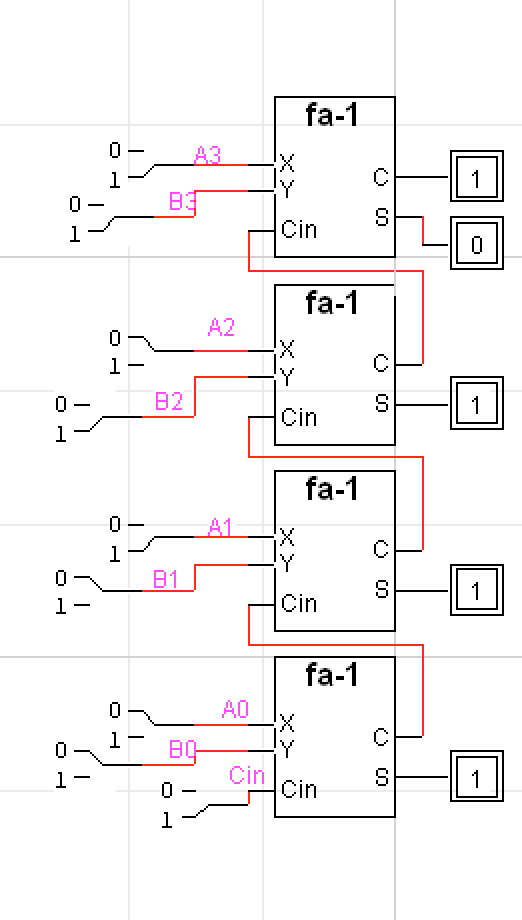
\includegraphics[width=150pt]{2at1}
					\caption{\label{fig:2atc} LogicWorks circuit test 1.}
				\end{figure}
			}
			\item{
				\[
					1010.0_2 + 0100.1_2 = 01110_2
				\]
				\[
					C_{\text{in}} = 0,
					A_0 = 0, A_1 = 1, A_2 = 0, A_3 = 1,
					B_0 = 0, B_1 = 0, B_2 = 1, B_3 = 0,
				\]
				\[
					S_0 = 0, S_1 = 1, S_2 = 1, S_3 = 1, C_{\text{out}} = 0
				\]

				Testing shown in figure \ref{fig:2atc1}.

				\begin{figure}[h]
					\centering
					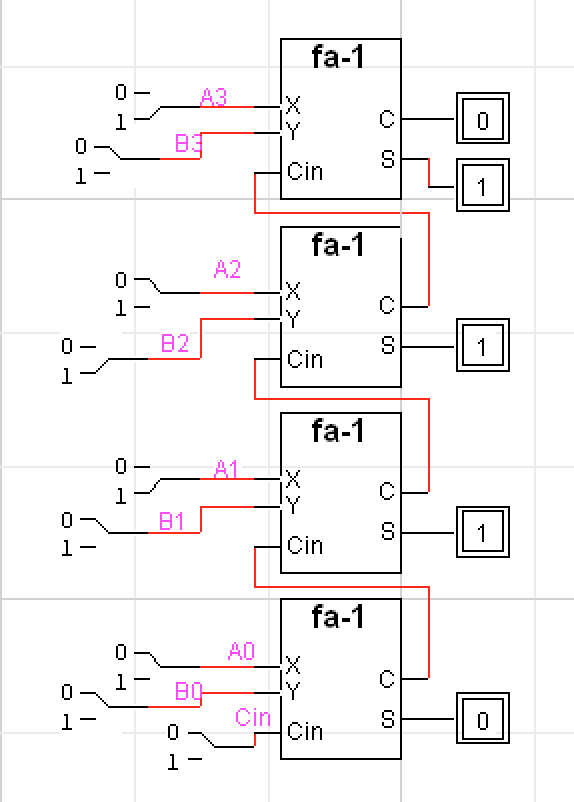
\includegraphics[width=150pt]{2at2}
					\caption{\label{fig:2atc1} LogicWorks circuit test 2.}
				\end{figure}
			}
			\item{
				\[
					0000.1_2 + 1111.1_2 = 10000_2
				\]
				\[
					C_{\text{in}} = 1,
					A_0 = 0, A_1 = 0, A_2 = 0, A_3 = 0,
					B_0 = 1, B_1 = 1, B_2 = 1, B_3 = 1,
				\]
				\[
					S_0 = 0, S_1 = 0, S_2 = 0, S_3 = 0, C_{\text{out}} = 1
				\]

				Testing shown in figure \ref{fig:2atc2}.

				\begin{figure}[h]
					\centering
					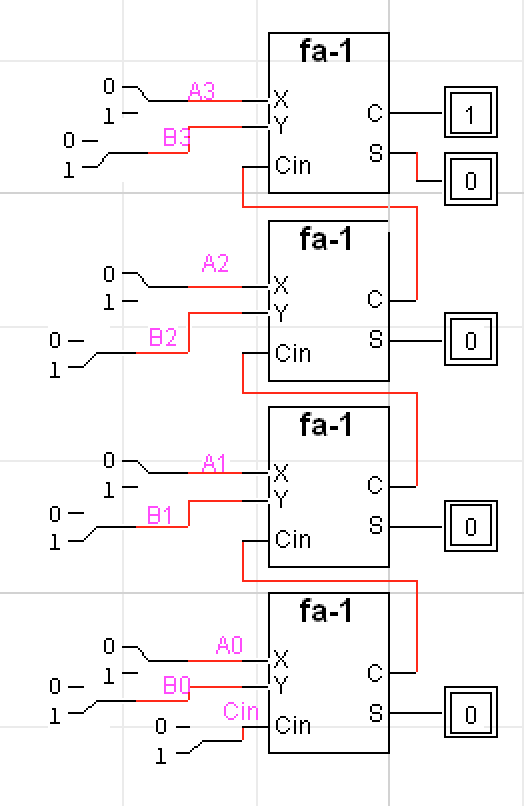
\includegraphics[width=150pt]{2at3}
					\caption{\label{fig:2atc2} LogicWorks circuit test 3.}
				\end{figure}
			}
		\end{enumerate}
	}
	\item{
		Figures \ref{fig:2btc}, \ref{fig:2btc1}, \ref{fig:2btc2} depict testing of the packaged circuit correlating to the above tests.

		\begin{figure}[h]
			\centering
			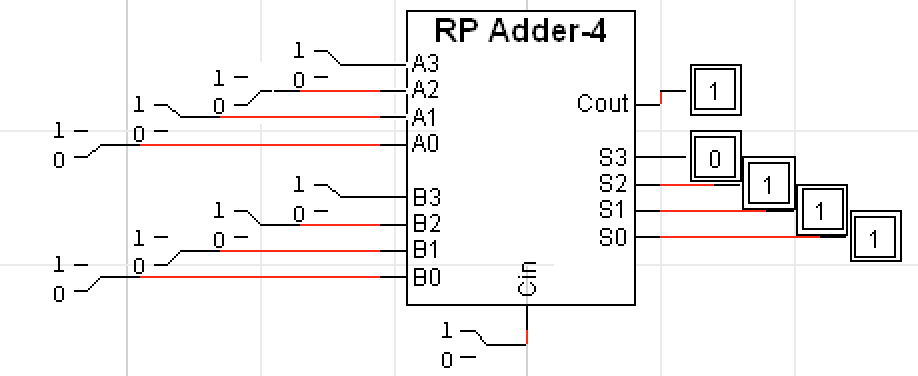
\includegraphics[width=200pt]{2pt1}
			\caption{\label{fig:2btc} LogicWorks circuit test 1.}
		\end{figure}
		\begin{figure}[h]
			\centering
			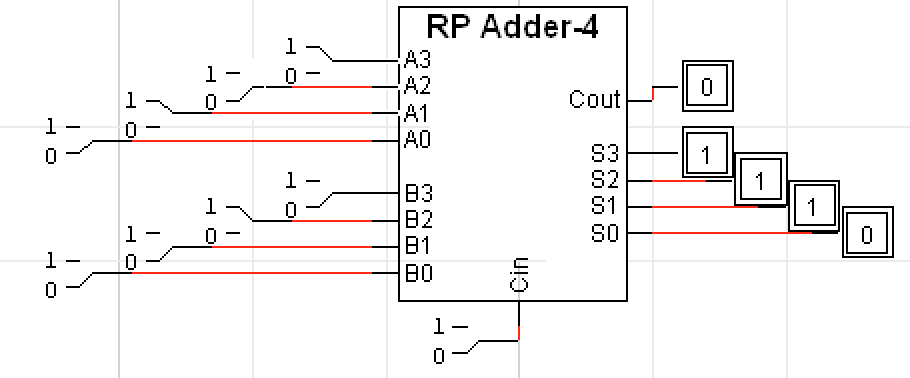
\includegraphics[width=200pt]{2pt2}
			\caption{\label{fig:2btc1} LogicWorks circuit test 1.}
		\end{figure}
		\begin{figure}[h]
			\centering
			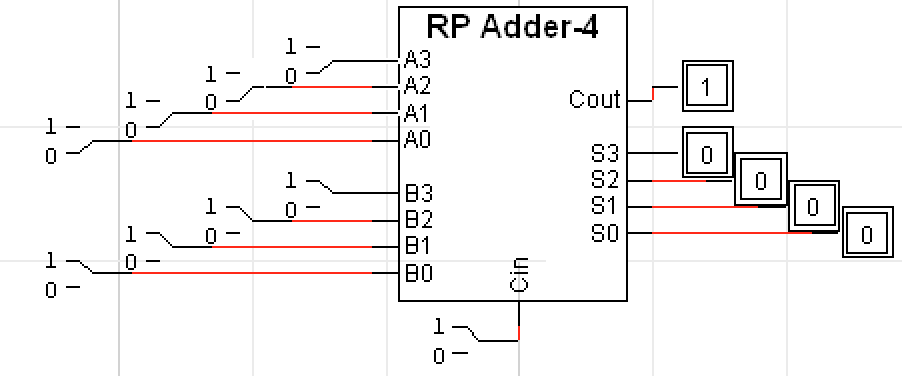
\includegraphics[width=200pt]{2pt3}
			\caption{\label{fig:2btc2} LogicWorks circuit test 1.}
		\end{figure}
	}
	\item{
		Test the longest propagation delays of your {\tt RP Adder-4} from the inputs to $C_{\text{out}}$ and $S_3$ (the highest bit of the sum) by setting $A_{3\text{-}0}$ and $B_{3\text{−}0}$ to make their sum to be 1111 and connecting $C_{\text{in}}$ to a clock.

		The circuit is shown in figure \ref{fig:2cc} and the output is shown in figure \ref{fig:2ct}. The testing shows a 1ns delay between $C_{\text{in}}$ and $S_0$, and a 2ns delay between $S_0$ and the next subcircuit ($S_1$), which continues between subcircuits. The delay between the last subcircuit ($S_3$) and its carry $C_{\text{out}}$ is 1ns. This totals 8ns. This is because each circuit has a 1ns delay between its $C_{\text{in}}$ input and its $S$ output, and an additional 1ns (2ns total) between its input and its carry output ($C$).

		Since this circuit is a ripple adder, each single-bit adder depends on the carry from the last single-bit adder. This leads to a 2ns delay for each additional bit. This type of circuit is $O(n)$ concerning gate delay (gates are operations) where $n$ is bits of the number.

		\begin{enumerate}[i.]
			\item{
				Figure \ref{fig:2cc} shows the testing circuit.
			}
			\item {
				Figure \ref{fig:2ct} shows the waveform of the testing circuit with $C_{\text{in}}$ as a reference line.
			}
			\item{
				The dalay from $C_{\text{in}}$ to $C_{\text{out}}$ is 8ns. The dalay from $C_{\text{in}}$ to $C_{\text{out}}$ is 7ns. The reason this differs by one nanosecond is that the carry ($C$) bit takes 2ns to compute while the $S$ bit takes only 1ns for each subcircuit. This is because the carry ($C$) bit is calculated with two gates in a row ($*$ then $+$), while the $S$ bit is calculated with a single gate ($\oplus$).

				The overall delay is caused by the dependency chain of each subsequent bit adder on the last carry bit output. Thusly this circuit is $O(n)$ operations (gate operations), meaning it scales in number of operations over time by the number of bits. The delay is $D_t = \sum\limits_{i=0}^n di$ where $d$ is the delay of each single-bit addition, in this case 2ns, $D_t$ is the total delay, and $n$ is the number of bits.
			}
		\end{enumerate}

		\begin{figure}[h]
			\centering
			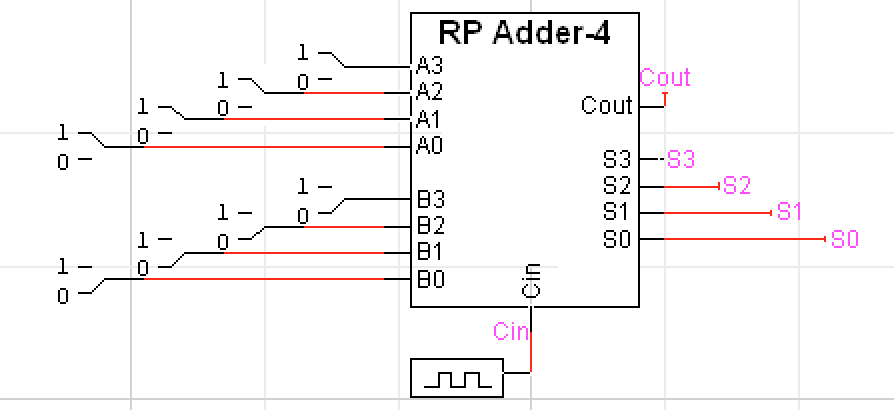
\includegraphics[width=200pt]{2pct}
			\caption{\label{fig:2cc} LogicWorks circuit delay test.}
		\end{figure}

		\begin{figure}[h]
			\centering
			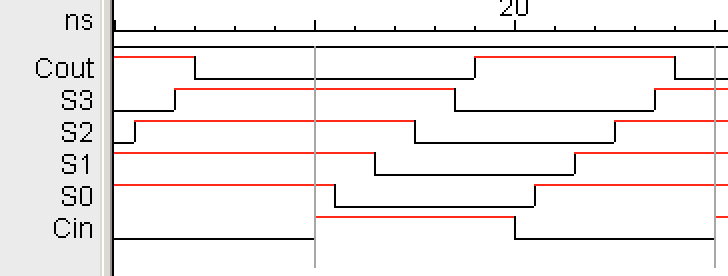
\includegraphics[width=200pt]{2ptt}
			\caption{\label{fig:2ct} Output showing delay.}
		\end{figure}
	}
\end{enumerate}

\section{Single-bit full adder with $p$ (carry propagation) and $g$ (carry generation) outputs.}

\begin{enumerate}[(a)]
	\item{
	Show the truth tables of $g$ (carry generation) and $p$ (carry propagation) of single-bit adder as functions of input $X$ and $Y$ (They do not depend on $C_{\text{in}}$).

		The truth table is shown in figure \ref{fig:3a}.

		\begin{table}[h]
		\centering
		\begin{tabular}{llll}
			$X$ & $Y$ & $g$ & $p$ \\ \hline
			0 & 0 & 0 & 0 \\
			0 & 1 & 0 & 1 \\
			1 & 0 & 0 & 1 \\
			1 & 1 & 1 & 0 \\
		\end{tabular}
		\caption{\label{fig:3a} Truth table for $g$ and $p$ for a single bit adder.}
		\end{table}
	}
	\item{
		Implement and pack the single-bit full adder with $g$ and $p$ outputs on LogicWorks. Show the testing of your packaged single-bit full adder with $g$ and $p$ outputs. (You need to test and show all 8 input cases.)

		Figure \ref{fig:3bc} shows the testing circuit for the packaged Single-bit full adder with $p$ (carry propagation) and $g$ (carry generation) outputs.

		Figure \ref{fig:3bt} shows the testing. As you can see $S$ is only on if one of the inputs $X$, $Y$, or $C_{\text{in}}$ is set or all are set, which is the same as the original single-bit adder, so it is correct. $p$ is correct because it should be on when either $X$ or $Y$ is on, but not both, and it is. $g$ is correct because it should be on if both $X$ and $Y$ are on, and it is. Thusly we can conclude that this single-bit adder with $p$ (carry propogation) and $g$ (carry generation) is correct. This shows all eight test cases are correct.

		\begin{figure}[h]
			\centering
			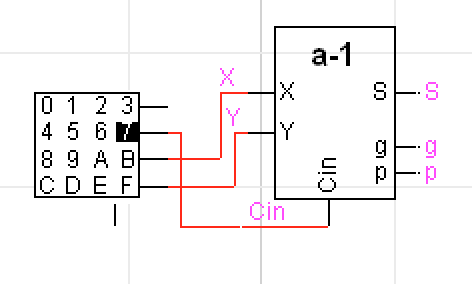
\includegraphics[width=200pt]{3pc}
			\caption{\label{fig:3bc} LogicWorks circuit.}
		\end{figure}

		\begin{figure}[h]
			\centering
			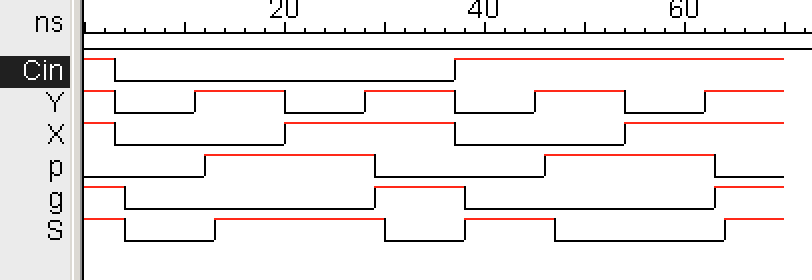
\includegraphics[width=200pt]{3pt}
			\caption{\label{fig:3bt} Waveform test.}
		\end{figure}
	}
\end{enumerate}

\section{4-bit carry look-ahead unit ({\tt LA-4})}

\begin{enumerate}[(a)]
	\item{
		Derive the Boolean expressions for carries $c1, \ldots, c4$ as functions of $g0, \ldots, g3$, $p0, \ldots, p3$, and $c0$.

		The formula for a carry bit is $C=g+pC_{\text{in}}$. For the first bit, carry in is given, and for the others, carry in is generated recersively based on the formula.
		\[
			C_1 = g_0+p_0C_0
		\]
		\[
			C_2 = g_1+p_1C_1 = g_1+p_1(g_0+p_0C_0)
		\]
		\[
			C_3 = g_2+p_2C_2 = g_2+p_2(g_1+p_1C_1) = g_2+p_2(g_1+p_1(g_0+p_0C_0))
		\]
		\[
			C_4 = g_3+p_3C_3 = g_3+p_3(g_2+p_2C_2) = g_3+p_3(g_2+p_2(g_1+p_1C_1)) = g_3+p_3(g_2+p_2(g_1+p_1(g_0+p_0C_0)))
		\]

		These can be simplified using the distributive property to derive:
		\[
			C_1 = g_0+p_0C_0
		\]
		\[
			C_2 = g_1 + p_1(g_0+p_0C_0) = g_1 + p_1g_0 + p_1p_0C_0
		\]
		\[
			C_3 = g_2+p_2(g_1+p_1g_0 + p_1p_0C_0) =  g_2 + p_2g_1 + p_2p_1g_0 + p_2p_1p_0C_0
		\]
		\[
			C_4 = g_3+p_3(g_2 + p_2g_1 + p_2p_1g_0 + p_2p_1p_0C_0) = g_3 + p_3g_2 + p_3p_2g_1 + p_3p_2p_1g_0 + p_3p_2p_1p_0C_0
		\]

		This second way is better because it is the sum of min-terms approach that we know can reduce gate dalays to a mamimum of 3.
	}
	\item{
		Derive the Boolean expressions for block carry generation $G$ and block carry propagation $P$ as functions of $g0, \ldots, g3$ and $p0, \ldots, p3$.

		The formula for $G$ and $P$ is $C_4=G+PC_0$, so using the $C_4$ derived in the previous step, we can see the following values for $G$ and $P$:
		\[
			G = g_3 + p_3g_2 + p_3p_2g_1 + p_3p_2p_1g_0
		\]
		\[
			P = p_3p_2p_1p_0
		\]
	}
	\item{
		Implement and pack the {\tt LA-4} unit in LogicWorks. Show the internal circuit of the unit.

		The circuit can be seen in figure \ref{fig:4c}.

		\begin{figure}[h]
			\centering
			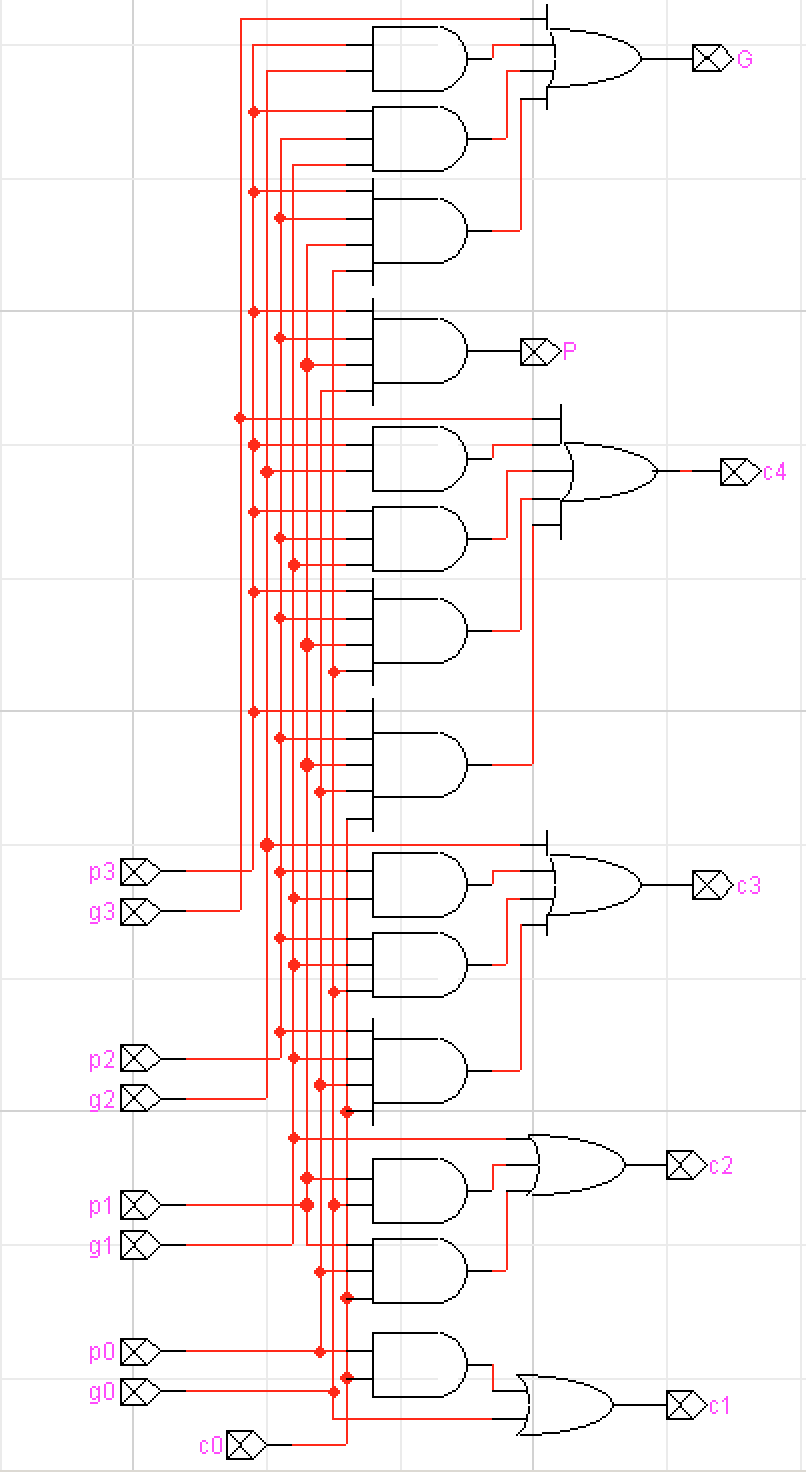
\includegraphics[width=200pt]{4c}
			\caption{\label{fig:4c} LogicWorks circuit implementation.}
		\end{figure}
	}
	\item{
		Show the testing of $c2$ of the {\tt LA-4}.

		Figure \ref{fig:4dc} shows the circuit in testing setup.

		Figure \ref{fig:4dt} shows the testing output wavelengths for all 32 applicable input combinations. $C_2 = g_1 + p_1(g_0+p_0C_0)$, so we can confirm the correctness of the circuit by showing that each value of $C_2$ is because $g_1$ or $p_1$ and either $g_0$ or $p_0$ and $C_0$. We can see for the first half when $C_0$ is off, that $C_2$ is off while $g_1$ and $p_1$ are off, and then turns on while $g_1$ is on. When $g_1$ is next off, $C_2$ reflects $g_0$ as $p_0$s value is of no importance whilst $C_0$ is off. It continues to follow the formula for the remainder of the wavelength and we can confirm it is correct.

		\begin{figure}[h]
			\centering
			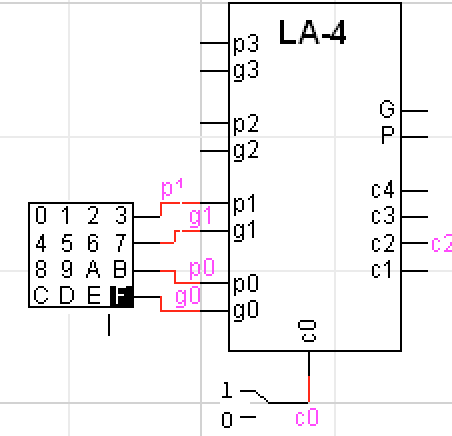
\includegraphics[width=200pt]{4ct}
			\caption{\label{fig:4dc} LogicWorks circuit implementation.}
		\end{figure}
		\begin{figure}[h]
			\centering
			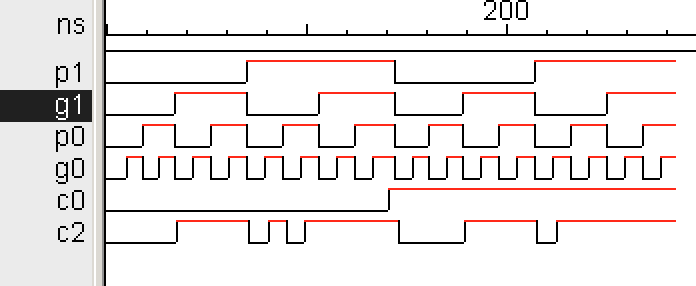
\includegraphics[width=200pt]{4t}
			\caption{\label{fig:4dt} Wavelength recording.}
		\end{figure}
	}
\end{enumerate}

\section{4-bit carry look-ahead adder}

\begin{enumerate}[(a)]
	\item{
		Implement the 4-bit carry look-ahead adder with inputs $A_{3\text{-}0}$ , $B_{3\text{-}0}$ and $C_{\text{in}}$ and outputs $S_{3\text{-}0}$, $C_{\text{out}}$, $G$ and $P$. Show the internal circuit of the adder.

		Figure \ref{fig:5ac} shows the internal circuit of the adder.

		\begin{figure}[h]
			\centering
			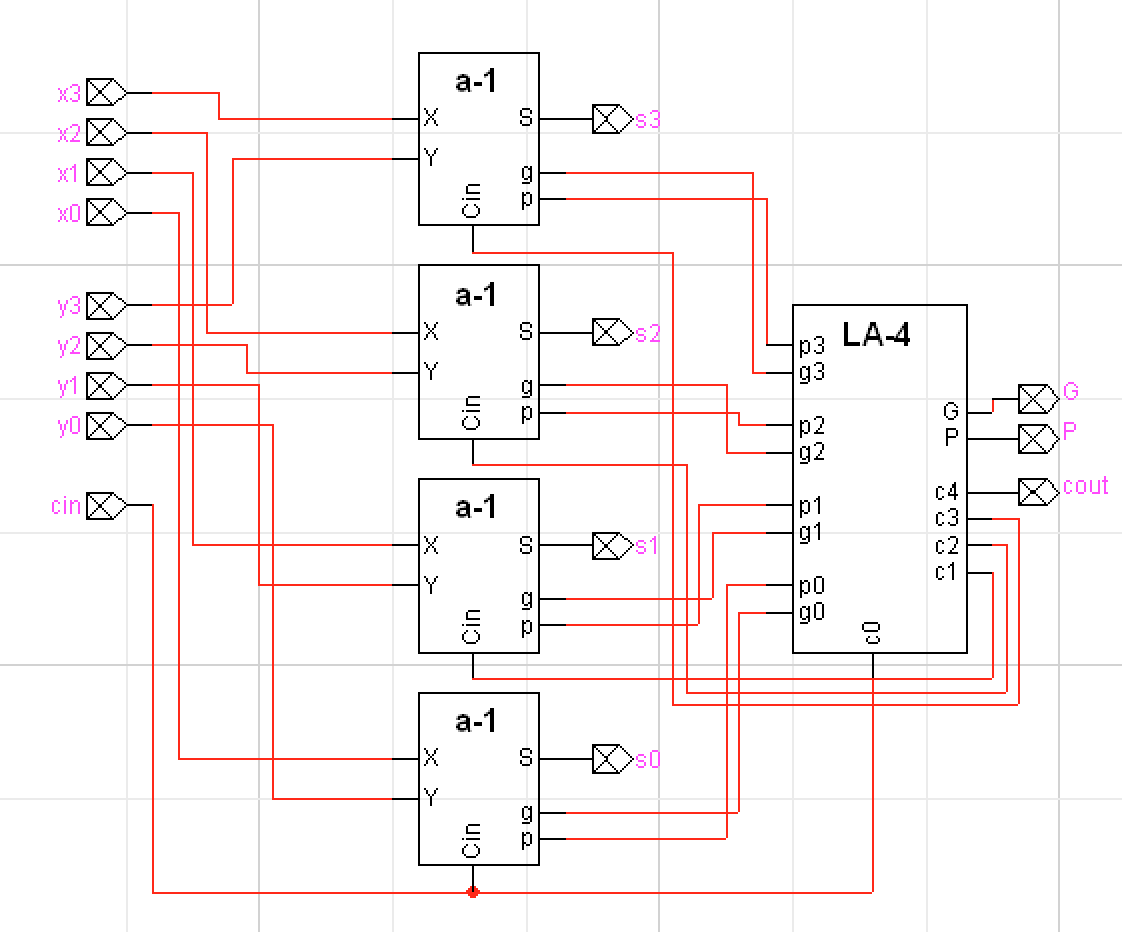
\includegraphics[width=200pt]{5c}
			\caption{\label{fig:5ac} LogicWorks circuit implementation.}
		\end{figure}
	}
	\item{
		Pack the 4-bit carry look-ahead and name it as {\tt Adder-4}. Show three test cases to demonstrate that your adder works correctly.

		The three cases for testing are as follows:
		\begin{enumerate}[1.]
			\item{
				\[
					1010.1_2 + 1100.1_2 = 10111_2
				\]
				\[
					C_{\text{in}} = 1,
					X_0 = 0, X_1 = 1, X_2 = 0, X_3 = 1,
					Y_0 = 0, Y_1 = 0, Y_2 = 1, Y_3 = 1,
				\]
				\[
					S_0 = 1, S_1 = 1, S_2 = 1, S_3 = 0, C_{\text{out}} = 1
				\]

				Testing shown in figure \ref{fig:5t}.

				\begin{figure}[h]
					\centering
					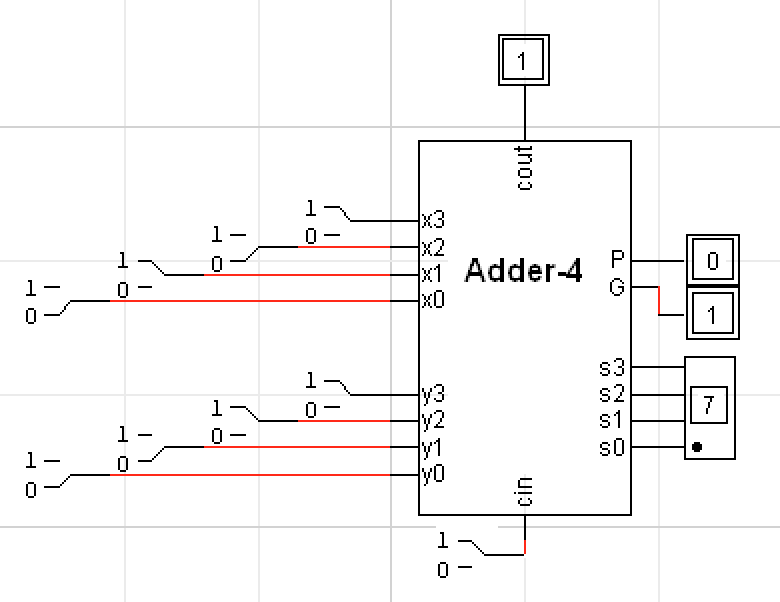
\includegraphics[width=150pt]{5t}
					\caption{\label{fig:5t} LogicWorks circuit test 1.}
				\end{figure}
			}
			\item{
				\[
					1010.0_2 + 0100.1_2 = 01110_2
				\]
				\[
					C_{\text{in}} = 0,
					X_0 = 0, X_1 = 1, X_2 = 0, X_3 = 1,
					Y_0 = 0, Y_1 = 0, Y_2 = 1, Y_3 = 0,
				\]
				\[
					S_0 = 0, S_1 = 1, S_2 = 1, S_3 = 1, C_{\text{out}} = 0
				\]

				Testing shown in figure \ref{fig:5t1}.

				\begin{figure}[h]
					\centering
					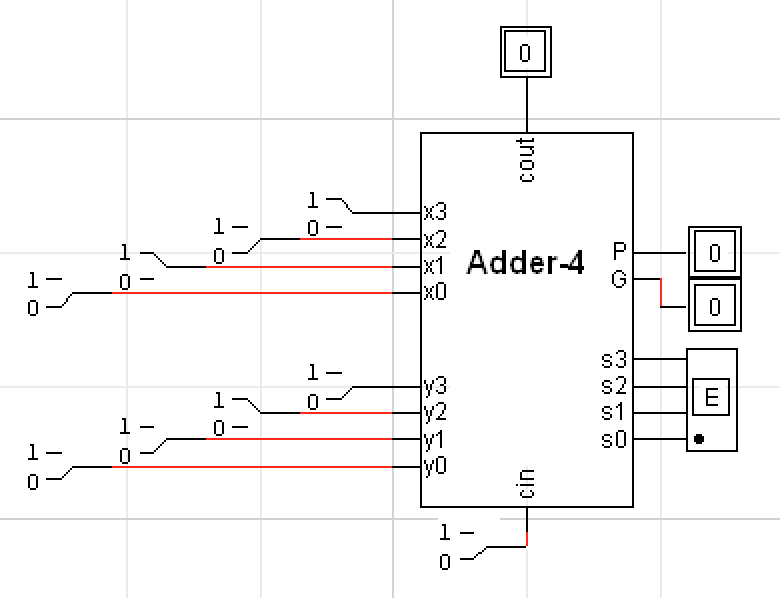
\includegraphics[width=150pt]{5t1}
					\caption{\label{fig:5t1} LogicWorks circuit test 2.}
				\end{figure}
			}
			\item{
				\[
					0000.1_2 + 1111.1_2 = 10000_2
				\]
				\[
					C_{\text{in}} = 1,
					X_0 = 0, X_1 = 0, X_2 = 0, X_3 = 0,
					Y_0 = 1, Y_1 = 1, Y_2 = 1, Y_3 = 1,
				\]
				\[
					S_0 = 0, S_1 = 0, S_2 = 0, S_3 = 0, C_{\text{out}} = 1
				\]

				Testing shown in figure \ref{fig:5t2}.

				\begin{figure}[h]
					\centering
					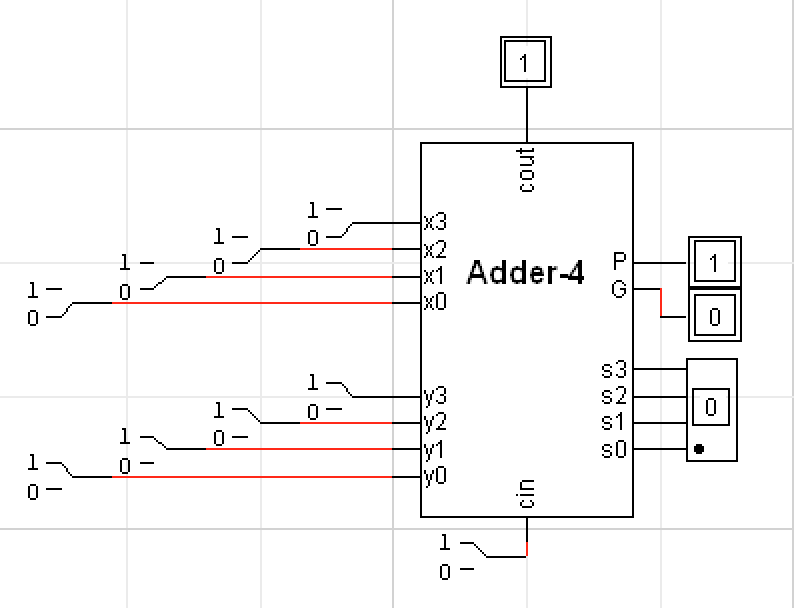
\includegraphics[width=150pt]{5t2}
					\caption{\label{fig:5t2} LogicWorks circuit test 2.}
				\end{figure}
			}
		\end{enumerate}
	}
	\item{
		Test the longest propagation delays of your carry look-ahead Adder-4 from the inputs to $C_{\text{out}}$ and $S_3$ (the highest bit of the sum) by setting $A_{3 \text{−} 0}$ and $B_{3 \text{−} 0}$ to make their sum to be 1111 and connecting $C_{\text{in}}$ to a clock.

		\begin{enumerate}[i.]
			\item{
				 Show your testing circuit.

				Figure \ref{fig:5dtc} depicts the circuit.

				\begin{figure}[h]
					\centering
					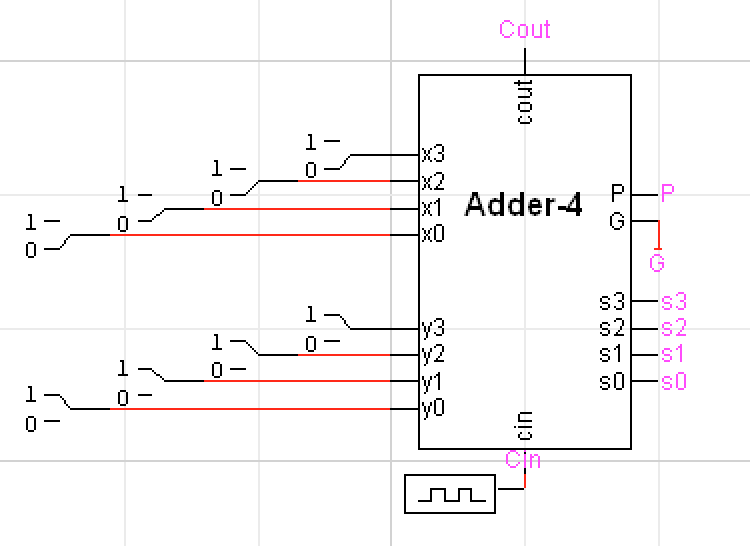
\includegraphics[width=150pt]{5dtc}
					\caption{\label{fig:5dtc} LogicWorks circuit test 2.}
				\end{figure}
			}
			\item{
			Show the waveforms of the inputs and outputs with the rising edges of $C_{\text{in}}$ as reference lines.

				Shown in figure \ref{fig:5dt}.

				\begin{figure}[h]
					\centering
					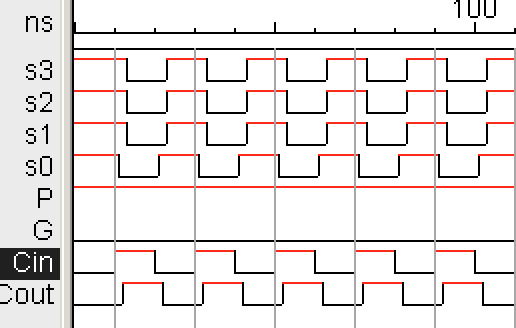
\includegraphics[width=150pt]{5dt}
					\caption{\label{fig:5dt} Wavelength}
				\end{figure}
			}
			\item{
				Show the propagation delays from $C_{\text{in}}$ to $C_{\text{out}}$ and $S_3$. Explain why these delays are such as you observed.

				The propogation delay from $C_{\text{in}}$ to $C_{\text{out}}$ is 3ns, while from $C_{\text{in}}$ to $S_3$ is 3ns. This is because the new way of calculating carry bits with the look-ahead unit does not depend on the previous cascading carry and is thusly $O(1)$ for $n$ bits. The $S$ takes an additional 1ns because it must wait for the cary bit to come back from the look-ahead.
			}
		\end{enumerate}
	}
\end{enumerate}

\end{document}
